\documentclass{article}

\usepackage[a4paper]{geometry}
\usepackage{graphicx}

\title{\textbf{Gitgroup Course Manager}\\
		\textit{Requirements, Design, and Planning}}
\author{Andrew Lalis\\
		\texttt{S3050831}}

\begin{document}

\maketitle

\tableofcontents

\newpage

\section{Introduction}
	Being a teaching assistant for both the introductory and advanced object oriented programming courses at the University of Groningen, I could not help but notice certain inefficiencies in how the courses are managed with regard to student groups and their associated git repositories.\\
	
	\noindent
	In particular, when the course is first created, all students must enter their information in a "sign-up form" (usually a Google Form). Then, a simple Python script is used to generate repositories for each student group. While quite straightforward and seemingly an elegant solution, limiting the automation of the course to the creation of repositories leads to a lot more difficulty in practice.\\
	
	\noindent
	It is given that some students will drop the course, and this leads to a lot of single-student groups, all of which must be dealt with manually on a case-by-case basis. As a teaching assistant for such courses, I see firsthand the issues this causes. First, teaching assistants such as myself are more reluctant to make modifications to existing groups, not only because it takes a significant amount of time and administrative effort to manually change repository configurations, but also because from an organizational perspective, it is a challenge to keep every single teaching assistant up-to-date. Additionally, the sources of information regarding each student group are quite scattered, and as of right now, there is no one single, definitive source of information on which all teaching assistants can rely. Having a way to unify all the different components of managing Github-utilizing courses is where the \textbf{Gitgroup Course Manager} gets its inspiration.
	
	\subsection{Vision}
		When this project is done, managing a course as the lead teaching assistant should be quick and painless, not just when creating student-group repositories, but also when making changes during the course's duration. The application should make basic tasks, such as moving students between groups or removing a student, trivial compared to the current state of affairs.\\
		
		\noindent
		While using this application, the teaching assistant should be able to find information about any student in a matter of seconds, rather than minutes, and changes should be made with only a few clicks, rather than spending a quarter of an hour navigating the settings page of Github.\\
		
		\noindent
		More specifically, the \textbf{Gitgroup Course Manager} is intended as a desktop application, to be used by the lead teaching assistant to perform all administrative tasks, and to serve as the definitive authority on the state of the course, in terms of current student groups and repositories.

\section{Requirements}
	While the vision provides a very subjective and vague overview of the application and its functionality, this section will go into more detail on the functional and non-functional requirements. The functional requirements will describe the explicit details of what the application should do, and the non-functional requirements will cover more abstract concepts such as reliability, security, and ease of use.\\
	
	\noindent
	However, before beginning to describe these requirements, it is important to define the different types of users of this application. Luckily this application is not very large, so all potential users of the system can be categorized into the following two groups.
	
	\subsection{Users}
	
		\begin{itemize}
			\item \textbf{Teaching Assistants (TA)} - Administrators of the application who have full access to all functionality and student group information.
		
			\item \textbf{Students} - Entities in the application, with no interactive permissions. Essentially, students make up the raw data used by the system, but may not make changes to the system.
		\end{itemize}
		
		\noindent
		To ease the process of defining functional requirements, some user stories are included here which describe in layman's terms the essential features of the application, which can then be extrapolated upon in later sections. Note that user stories are written from the point of view of one of the two user types given above, and each story will identify this by starting with, \textit{"As a ..., I want ..."}. However, the vast majority of user stories will be from the teaching assistant's perspective, obviously.
		
		\subsubsection{User Stories}
			\begin{enumerate}
				\item As a teaching assistant, I want to be able to use a Google Form's CSV output to generate a list of student groups, because this is the first step in initializing a new course.
				
				\item As a teaching assistant, I want to let students enroll for groups using Nestor's built-in group enroll feature, because this makes enrollment much easier for students.
				
				\item As a teaching assistant, I want the application to automatically assign students to groups based on their preferred partners, because this is a good feature to have for the students' benefit.
				
				\item As a teaching assistant, I want to generate repositories for newly generated groups, possibly on a case-by-case basis, because this gives me the same precision as manually creating repositories, while also providing the ease of complete automation if preferred.
				
				\item As a teaching assistant, I want to be able to view all students, the group they're in, and what repository is related to that group, if any, because this is needed for basic day-to-day productivity for all teaching assistants.
				
				\item As a teaching assistant, I want to have access to all a student's information, and have the ability to modify it, because there are cases where students may incorrectly enter personal information.
				
				\item As a teaching assistant, I want to be able to create a new empty student group, because this functionality is needed for when students are late in signing up for the course, or in other extraneous situations.
				
				\item As a teaching assistant, I want to be able to remove empty student groups (including any associated repositories), because this is necessary housekeeping for an administrator of the course.
				
				\item As a teaching assistant, I want to be able to add or remove a student from a group, because this is necessary when some students leave the course, or new ones join.
				
				\item As a teaching assistant, I want to be able to assign a teaching assistant team to a group, so that they are responsible for micro-management of that group's activities and grades.
				
				\item As a teaching assistant, I want to filter student groups by which teaching assistant they are assigned to, because this makes management easier for other teaching assistants.
				
				\item As a teaching assistant, I want to see all open issues and pull requests on every group's repository, so that it is easier to view all open issues in one place, as opposed to the current workflow on Github.
				
				\item As a teaching assistant, I want to provide short answers to simple issues from the application itself without having to navigate to the issue on Github's website.
				
				\item As a teaching assistant, I want to be able to see the time at which a pull request was made, so that it is easy to determine if the pull request passed a certain deadline or not.
				
				\item As a teaching assistant, I want to add branch protection rules and continuous integration to a branch for many groups at once, since this is by far the most tedious part of manually creating new repositories.
				
				\item As a teaching assistant, I want the application to save everything permanently, so that even if, for example, a group is removed, their repository is not simply deleted but instead just archived, and individual student information is not deleted but archived.
				
				\item As a teaching assistant, I want use the mapping of TA teams to student teams to create spreadsheets (using Google Sheets) which can be filled in with grades for each student group.
				
				\item As a teaching assistant, I want to store filled-in grade sheets so that I can look up a student group's grade for a particular assignment, or even a particular category in an assignment, and make changes later if needed.
				
				\item As a teaching assistant, I want to be able to export a CSV file containing the student group grades so that it can be uploaded to Nestor and made official.
				
				\item As a teaching assistant, I want to retrieve some statistics about past assignments in terms of average grades, average grades per teaching assistant, per group, etc. because this will help in identifying cases where there is a discrepancy grading standards that can be addressed.
				
				\item As a student, I want to provide my personal information to this course as few times as possible, because by complicating the sign-up process, more students are discouraged from signing up.
				
				\item As a student, I want to be certain that my information is stored securely.
			\end{enumerate}
	
	\subsection{Functional Requirements}
		As can be seen from the large amount of user stories that can be generated about this application, simply listing all the functional requirements is a rather cumbersome task. To better organize the requirements and make the list conceptually easier to understand, the requirements will be split into several categories based on the section of the application to which they apply.
		
		\subsubsection{Course Initialization}
			In this first section, the requirements will be listed which pertain directly to course initialization, or the basic functionality that must be present for starting the course, creating groups and repositories, etc.
			
			\begin{itemize}
				\item The application can parse CSV data about students from a Google Forms sign-up form, or from Nestor's group-enroll mechanic.
				
				\item A list of groups can be generated from the parsed information about students, taking into account each students' preference for partners.
				
				\item The application can automatically generate all repositories for newly generated groups, including adding branch protection and continuous integration to a branch.
				
				\item Students are automatically invited to the repository for the group they're assigned to.
				
				\item The application can parse CSV data about teaching assistants to build a list of all teaching assistants in the course, and optionally, if they are grouped together into teams.
				
				\item A teaching assistant team can be assigned to each student group.
			\end{itemize}
			
		\subsubsection{Course Management}
			In this section will be found all the requirements for general management of the course, for the duration of the course.
			
			\begin{itemize}
				\item The user (teaching assistant) is able to view a list of students in the course, a list of student groups, a list of repositories, a list of teaching assistants, and a list of teaching assistant groups, such that it is possible to view a list of all entities in the application.
				
				\item The teaching assistant may modify some information of an entity, while other information may be forbidden from editing.
				
				\item Student groups can be created, edited (changing the members in a group), or removed by a teaching assistant.
				
				\item The application should be able to provide a list of all open issues in all student group repositories, and a list of all open pull requests (including time and date, especially with regard to pull requests).
				
				\item Teaching assistants may provide simple replies to issues from within the application, and if that is not enough, a link is provided to the issue online.
				
				\item A command prompt should be available for advanced users to execute commands separately than through the interface.
			\end{itemize}
			
		\subsubsection{Grading}
			In this section, there are a few requirements specific to grading which can be addressed separately from others, and in fact, the grading system will be implemented as a sub-system of the main application, as will be seen in the design section of this document.
			
			\begin{itemize}
				\item The application can generate grading sheets for a certain assignment, given the number of categories (and grading weights), and that each group is assigned a teaching assistant team.
				
				\item The application can parse filled-in grading sheets for a certain assignment, and stores each group's grade for that assignment.
				
				\item A CSV file can be exported, containing grades in such a format as to be accepted by Nestor's grade center.
				
				\item Reports can be generated for students or student groups, giving a detailed overview of the grades and any comments that were given along with the grade itself.
			\end{itemize}
	
	\subsection{Non-Functional Requirements}
		For this application, because it will function as a desktop application, does not need to concern itself with the performance issues which are commonplace in web applications. Additionally, by operating on the local system, it does not suffer from uptime issues that web apps can deal with. Therefore, the non-functional requirements for this application are simplified to a subset of what many modern projects must deal with.
		
		\begin{itemize}
			\item \textbf{Ease of use} - The application should be intuitive to use, and have necessary redundancies such that the user's interactive experience is similar to many other desktop applications. However, due to the time constraints, this may not be fully achieved.
			
			\item \textbf{Data safety} - All changes to the data should be permanent, so that when the user sees an updated value in the interface, the user is confident that the value has been saved to the hard drive, and will persist so long as the computer does.
			
			\item \textbf{Data security} - While not quite as large of an issue as it would be with a web application, steps should be taken to ensure a high level of security, especially with regard to student grades, so that data is consolidated in one place, accessible only to the teaching assistant.
		\end{itemize}

\section{Design}
	The application can be divided into three main conceptual components, the initialization of a new course, the management of an existing course, and grade recording. These three modules form the basis of the application design.
	
	\begin{figure}[h]
		\centering
			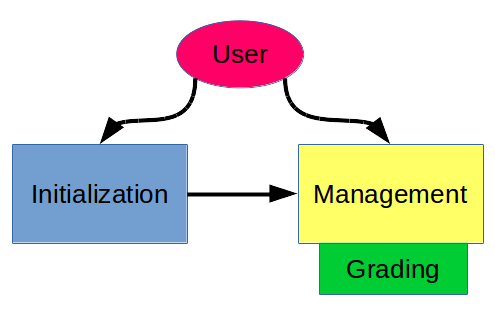
\includegraphics[width=0.4\textwidth]{image/modules.png}
			\caption{The modules in this application, as well as the user's starting point.}
	\end{figure}
	
	\noindent
	As shown in Figure 1, the user may begin the application either by initializing a new course, or continuing directly to the management module. From within the management module, the user may interact with the grading module.
	
	\subsection{Initialization Module}
		In this first module, the teaching assistant is prompted to enter all information needed to initialize a course. This includes:
		
		\begin{itemize}
			\item The Github Organization name.
			
			\item The teaching assistant's access token.
			
			\item The name of the repository which contains the assignments for the course.
			
			\item Data about teaching assistants (Names, emails, Github usernames, etc.).
			
			\item Student CSV data.
		\end{itemize}
		
		\noindent
		With this information, it is then possible to let the application populate its database with all the student and teaching assistant information, and generate groups based on student preference. From there, the user is directed to the management module, wherein they will have access to all entities (students, groups, teaching assistants, etc.), and where most functionality of the application is implemented.
		
	\subsection{Management Module}
		In the management module is where the user will spend the majority of their time with the application. It will consist of three sub-modules: the command-line interface, the entity list view, and the entity detail view.
	
		\begin{figure}[h]
			\centering
				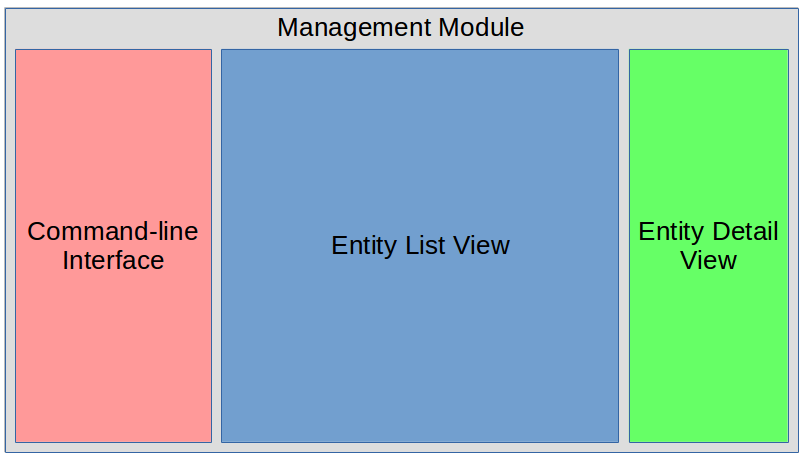
\includegraphics[width=0.6\textwidth]{image/managementModule.png}
				\caption{The management module.}
		\end{figure}
		
		\subsubsection{Command-line Interface}
			In this section of the managment module, the user will be able to see program output in a console-like format, with some extra logging details available. The user will also be able to enter text commands in an input field, as a means of being able to perform all actions without having to navigate the interface. Additionally, this interface can serve as a useful debugging tool during development, as it gives the developer the ability to test all functiontionality of the application via the command line, instead of being forced to create all the user interfaces to gain access to abstract commands.
			
		\subsubsection{Entity List View}
			This view will make up the majority of the management module's screen space, and is intended to command the majority of the user's attention. It is in this view that the user will be able to see a list of entities (students, student groups, teaching assistants, repositories, etc.) and interact with them. Selecting an entity in this list will display more detailed information about it in the entity detail view, which is discussed in the next section.\\
			
			\noindent
			Context menus will be used to provide the majority of functionality, so that when a user right-clicks on any entity, that entity will provide a list of actions which could be done to it, and clicking any one of the associated menu buttons will trigger some action. Multiple entities may be selected at once, and then only certain \textit{multiple-entity actions} may be performed, such as removing the entity, assigning multiple students to the same group, etc.
		
		\subsubsection{Entity Detail View}
			In this section will be shown all the detailed information about an entity which, in some cases, cannot all be displayed in the entity list view. Inside the entity detail view, it will be possible to edit the properties of an entity which could not be changed in the entity list view.

	\subsection{Grading Module}
		This module, accessed in the same view as the management module, will provide additional functionalities that help a teaching assistant to organize grading. In particular, this module will provide the following facilities:
		
		\begin{itemize}
			\item \textbf{Assignment sheet creation} - Guides the user through the creation of a grading sheet which can be filled in by teaching assistants during grading, with one or more weighted categories.
			
			\item \textbf{Assignment sheet reading} - The user may provide a filled-in grading sheet which was created previously in the application, and use this for recording the grades of student groups.
			
			\item \textbf{Grade reports} - The application will be able to generate PDF reports for individual students or student groups, which contain all grades, comments and other feedback for the included students.
			
			\item \textbf{Export for Nestor} - Ideally, grades managed in this application should be able to be transferred to Nestor in only a few clicks, and this can be done by generating a CSV sheet which can be uploaded to Nestor.
		\end{itemize}

\newpage
\section{Planning}
	With a solid plan for the application, as well as the lack of a way to perform comprehensive large-scale testing of the system as a whole, the waterfall model will be used for development of this project. While many software development platfoms are starting to use "Agile" development models in which a minimum viable product is released in a matter of one or two weeks, an application like this is not really viable until the majority of the requirements mentioned in this document are met. Otherwise, it is simply more effective to manually manage a course's student groups and repositories.\\
	
	\noindent
	Therefore, the project will be divided into three phases of development: Planning and Design, Application Development, and finally, Testing and Bug Fixing. This document itself represents the majority of the Planning and Design phase, and then soon the project will move into the development phase, where the design is fixed while the product is being made. Once all requirements in this document are met, the project has reached the Testing and Bug Fixing phase, in which the application is tested with large data sets and many extraneous situations to ensure that normal use will not result in critical errors if and when the application is deployed into real-world use.

\end{document}